\subsection{Beschreibung der Komponenten}
\subsubsection{Rampen}
Eine Rampe dient zur Aufnahme und Ausgabe von Paketen. Sie kann bis zu 4 Paketen aufnehmen. Es gibt eine Eingangsseite und eine Ausgangsseite. Die Pakete bewegen sich nur in eine Richtung. Jeder Slot wird mit einer Lichtschranke überwacht und ausfahrbare Bolzen vereinzeln die Pakete. Ein Micaz Controller ist die Agentenplattform. 
\begin{figure}[h!]
	\centering
		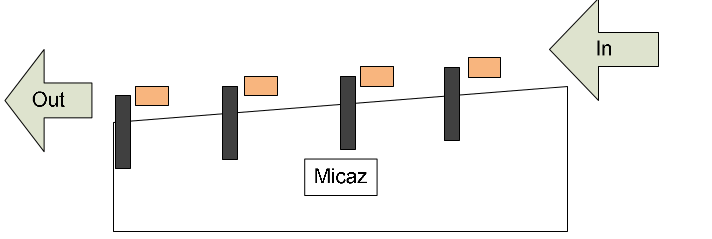
\includegraphics[width=0.9\textwidth]{SkizzeRampe.png}
	\caption{Skizze einer Rampe\cite{Stasch:Hahn}}
	\label{SkizzeRampe}
\end{figure}

\subsubsection{Mikrocontroller}
Ein Mikrocontroller ist ein kleiner Computer auf einem einzelnen Halbleiter-Chip. Dazu geh\"oren ein Prozessor,
der Programme ausf\"uhren kann, Arbeits- und Programmspeicher sowie Schnittstellen, die eine Kommunikation mit 
der Umgebung erm\"oglichen sog. Peripheriefunktionen \cite{Wikibooks:2014:Online}. Mit ihnen lassen sich komplexe
Aufgaben l\"osen, f\"ur die sonst ein aufw\"andiger Schaltungsaufbau notwendig w\"are. Standardm\"a{\ss}ig sind folgende Bestandteile in Mikrocontrollern integriert:
CPU, SRAM und Flash-Speicher f\"ur den Programmcode. Weiterhin bieten MCs analoge und digitale Ports, 
mehrere AD/DA-Wandler, Timer und Schnittstellen zur Kommunikation mit der Außenwelt \cite[vgl.]{Viktor:Seib:2014:Online}.
In der nachstehenden Abbildung ist der allgemeine schematische Aufbau eines Mikrocontrollers in folgender Abbildung dargestellt.
\begin{figure}[h!]
	\centering
		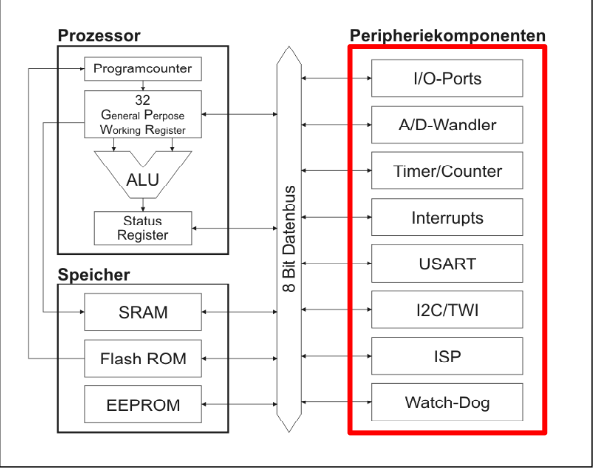
\includegraphics[width=0.9\textwidth]{Aubau_eines_Mikrocontrollers.png}
	\caption{schematischer Aufbau eines Mikrocontrollers \cite{habil:Ostermeye:2014:Online}}
	\label{Aufbau eines Mikrocontrollers}
\end{figure}

\begin{itemize}
\item Prozessor (CPU)
\begin{itemize}
          \item Arithmetic Logic Unit, kurz ALU (Rechenwerk)
          \item 32 GPIO-Register (Arbeitsregister f\"ur ALU)
          \item Programmcounter (Programmposition)
					\item Statusregister (Status der aktuellen Operation) 
\end{itemize}
\item Speicher
\begin{itemize}
          \item SRAM Datenspeicher (Static Random-Access Memory)
					\item Flash ROM Programmspeicher (Read Only Memory)
					\item EEPROM Festspeicher (Electrically Erasable Programmable Read-Only Memory)
\end{itemize}
\item Peripheriekomponenten
    \begin{itemize}
          \item I/O-Ports Prim\"arfunktion der Pins (Ein- und Ausg\"ange)
          \item A/D-Wandler (Einlesen von analogen Spannungen)
          \item Timer/Counter (Zeitintervall-/PBM-Generator)
					\item Interrupts (Programmunterbrechungsroutinen)
					\item USART, I2C/TWI und SPI (Kommunikationsschnittstellen)
					\item Watch-Dog (Absicherung gegen Systemfehler)
					\item ISP (Schnittstelle zum \"{U}bertragen des kompilierten Programms)
	\end{itemize}
\end{itemize}
Mikrocontroller sind im heutigen Leben weit verbreitet und es gibt eine große Anzahl von Herstellern, die Mikrocontroller anbieten.
Im Folgenden werden einige Hersteller mit ihren MC-Familien beispielhaft aufgef\"uhrt:
\begin{itemize}
\item Intel (8051-Serie)
\item Renesas (H8)
\item Zilog (Z8)
\item Microchip (Pic)
\item Freescale (fr\"uher Motorola) (68HC08 bzw. 68HCS08)
\item Atmel (AVR, 8051-Serie)
\end{itemize}
F\"ur das Projekt FAISE wurde die Atmel-Serie eingesetzt. Es sind Mikrocontroller mit erweiterten Peripherien und Funktionen, 
die auf der 8-Bit-AVR-Architektur basieren. Bei AVR handelt es sich um einen RISC-Kern, der an der Universit\"at von Trondheim 
in Norwegen entwickelt und von Atmel aufgekauft wurde. Die CPU besitzt 32 allgemeine 8-Bit Register (general purpose registers) 
und ist in der Lage in einem einzigen Taktzyklus Daten aus zwei beliebigen Registern in die ALU zu laden, diese zu verarbeiten 
und das Ergebnis in einem beliebigen Register zu speichern \cite[vgl.]{Viktor:Seib:2014:Online}. Die Konfiguration eines Atmega 8 der Firma Atmel sieht so aus:
\begin{figure}[h!]
	\centering
		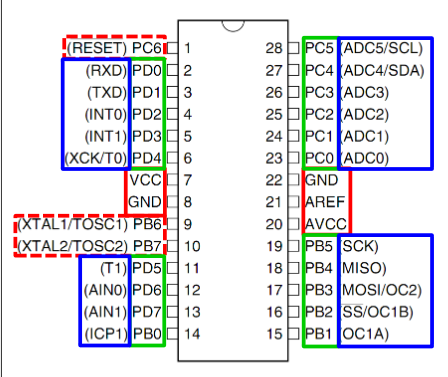
\includegraphics[width=0.9\textwidth]{Atmel8.png}
	\caption{Atmel 8 \\ \url{(http://www.ids.tu-bs.de/tl\_files/Lehre/Vorlesungen/Simulation2/Einfuehrung\_in\_die\_MC\_Programmierung\_Teil1.pdf)}}
	\label{Atmel 8}
\end{figure}
\begin{figure}[h!]
	\centering
		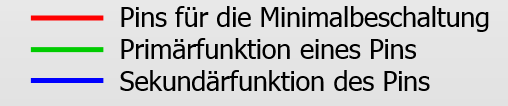
\includegraphics[width=0.9\textwidth]{LegendeAtmel8.png}
	\caption{Atmel 8 \url{(http://www.ids.tu-bs.de/tl\_files/Lehre/Vorlesungen/Simulation2/Einfuehrung\_in\_die\_MC\_Programmierung\_Teil1.pdf)}}
	\label{Legende Atmel8}
\end{figure}
\begin{itemize}
\item Pins f\"ur die Minimalbeschaltung
\begin{itemize}
          \item Spannungsversorgung
          \item Referenzspannung/Taktgeber
          \item Reset      
					\end{itemize}
\item Prim\"arfunktion eines Pins
\begin{itemize}
          \item Ein- bzw. Ausgang
					\end{itemize}
\item Sekund\"arfunktion des Pins
\begin{itemize}
          \item A/D-Wandlereingang
          \item Ext. Interrupt
          \item PBM-Ausgang   
\end{itemize}
\end{itemize}
F\"ur die Programmierung der AVR-Controller gibt es eine kostenlose Entwicklungsumgebung AVR-Studio, die das Einbinden des Compilers problemlos erlaubt.

\paragraph{ Sensorik und Aktorik}
Hauptziel der Teilgruppe Materialfluss ist das Management von Paketen auf einer Rampe.
Die Aufgabe der Sensorik ist dabei, dass die mit Lichtschranken ausgestatteten Rampen Pakete detektieren und auf \"Anderungen der Positionen der Pakete reagieren.
Die Lichtschranken bestehen aus einer Lichtstrahlenquelle (dem Sender) und einem Sensor (dem Empf\"anger) f\"{u}r diese Strahlung.
Als Lichtquelle kommt Infrarotlicht zum Einsatz und der Vorteil besteht in der einfachen Einstellung des Sensorsystems durch den
sichtbaren Lichtfleck. Das Funktionsprinzip der Lichtschranke besteht darin, den sich  \"andernden Zustand durch die Lichtintensit\"at mit dem Sensor zu registrieren. 
Die Rampen werden auf Hardwareebene um eine Aktorik zum Arretieren der Kisten erg\"anzt. Diese Aktoren (in unserem Fall die
eingesetzte Bolzenpaare) sind f\"ur das Ausf\"uhren von Bewegungen zust\"andig.
Sie sind aktive Stellelemente, die in der Antriebs- und Steuerungstechnik vom  Mikrorechner angesteuert werden, um das Verhalten des Prozesses durch das vom Sensor kommende Signal in einer gew\"{u}nschten Weise zu erm\"oglichen. In dieser allgemeinen Darstellung stehen die 
Ausgangssignale eines Sensors und die Stellsignale der Aktoren mit einem
Informationsverarbeitungssystem (IVS) in Verbindung.